% !TeX spellcheck = russian-aot
%\documentclass[12pt,a4paper,draft]{article}
%\usepackage{cmap}
%\usepackage[utf8]{inputenc}
%\usepackage[T2A]{fontenc}
%\usepackage[english,german,russian]{babel}
%\usepackage{amsmath}
%\usepackage{amsfonts}
%\usepackage{amssymb}
%\usepackage[final]{graphicx}
%\DeclareGraphicsExtensions{.jpg,.png}
%\graphicspath{{pictures/}} % путь к графическим файлам. Пусть они помещаются в подкаталог pictures текущего каталога
%\usepackage[figurename=Рисунок,labelsep=period]{caption}
%\usepackage{float}
%\usepackage{indentfirst}
%\usepackage[pdftex,left=2.5cm,right=2.5cm,top=3cm,bottom=3cm]{geometry}
%\usepackage[obeyDraft]{todonotes}
%\usepackage[hidelinks,draft=false]{hyperref}
%\frenchspacing
%\pdfcompresslevel=9

\documentclass[a4paper,12pt]{article}
\usepackage[utf8]{inputenc}
\usepackage[T2A]{fontenc}
\usepackage[english,russian]{babel}
\usepackage{natbib}
\usepackage[final]{graphicx}
\DeclareGraphicsExtensions{.jpg,.png}
\graphicspath{{pictures/}}
\usepackage{float}
\usepackage{amsmath}
\usepackage{pgfplots}
\usepackage{color} %% это для отображения цвета в коде
%\usepackage{listings} %% собственно, это и есть пакет listings




%\setmonofont{Consolas} %to be used with XeLaTeX or LuaLaTeX
\definecolor{bluekeywords}{rgb}{0,0,1}
\definecolor{greencomments}{rgb}{0,0.5,0}
\definecolor{redstrings}{rgb}{0.64,0.08,0.08}
\definecolor{xmlcomments}{rgb}{0.5,0.5,0.5}
\definecolor{types}{rgb}{0.17,0.57,0.68}

\usepackage{listings}
\lstset{
language=[Sharp]C,
captionpos=t,
%numbers=left, %Nummerierung
%numberstyle=\tiny, % kleine Zeilennummern
frame=lines, % Oberhalb und unterhalb des Listings ist eine Linie
showspaces=false,
showtabs=false,
breaklines=true,
showstringspaces=false,
breakatwhitespace=true,
escapeinside={(*@}{@*)},
commentstyle=\color{greencomments},
morekeywords={partial, var, value, get, set},
keywordstyle=\color{bluekeywords}\bf,
stringstyle=\color{redstrings},
basicstyle=\ttfamily\small,
extendedchars=\true
}

\usepackage{caption}
\DeclareCaptionFont{white}{\color{white}} %% это сделает текст заголовка белым
%% код ниже нарисует серую рамочку вокруг заголовка кода.
\DeclareCaptionFormat{listing}{\colorbox{gray}{\parbox{\textwidth}{#1#2#3}}}
\captionsetup[lstlisting]{format=listing,labelfont=white,textfont=white}


\usepackage{ctable}%для таблиц
\captionsetup[table]{justification=raggedleft,singlelinecheck=off}

\pgfplotsset{boble/.style = {blue}}
\pgfplotsset{insert/.style = {red}}
\pgfplotsset{qsort/.style = {green}}

%%%%%%%%%%%%%%%%%%%%%%%%%%%%%%%%%%%%%%%%%%%%%%%%%%%%%%%%%%%%%%%%%%%%%%%%%%%%%%%%%%%%%%%%%%%%%%%

\begin{document}
\begin{titlepage}
	\centering
    \begin{figure}[H]
    	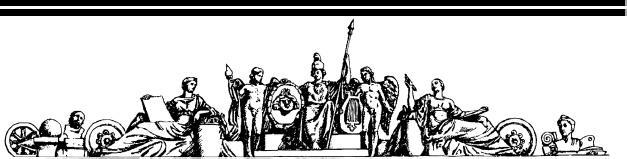
\includegraphics[scale=1.2]{photo}
   	\end{figure}
	{\scshape Министерство образования Российской Федерации
Московский Государственный Технический Университет им. Н.Э. Баумана \par}
	\vspace{4cm}
	{\scshape\Large Отчёт по лабораторной работе № 1\par}
    {\scshape\Large По курсу: "Анализ алгоритмов"\par}
	{\scshape\Large\bf Тема:"Алгоритмы сортировок"\par}
    \vspace{4cm}
    {\flushright Студент: Орехова Е.О. ИУ7-51\par
    \flushright Преподаватель: Волкова Л.Л.\par}
    \vspace{3cm}
% Bottom of the page
	{\large \today\par}
\end{titlepage}

\def\contentaname{Содержание}
\tableofcontents %Вывод содержания
\clearpage

\section{Постановка задачи}
    В ходе выполнения лабораторной работы необходимо вывести трудоёмкость трёх алгоритмов сортировок, сравнить полученные данные с экспериментальными. Сделать выводы.

\section{Сортировка пузырьком}
	\subsection{Идея}
	Алгоритм состоит из повторяющихся проходов по сортируемому массиву. За каждый проход элементы последовательно сравниваются попарно и, если порядок в паре неверный, выполняется обмен элементов. Проходы по массиву повторяются N-1 раз или до тех пор, пока на очередном проходе не окажется, что обмены больше не нужны, что означает — массив отсортирован. При каждом проходе алгоритма по внутреннему циклу, очередной наибольший элемент массива ставится на своё место в конце массива рядом с предыдущим «наибольшим элементом», а наименьший элемент перемещается на одну позицию к началу массива
	\subsection{Реализация}
	\begin{lstlisting}[label=some-code,caption={Сортировка пузырьком.}]
	static private void boble(ref int [] arr, int len)
	{
		int change;
		for (int j = 0; j<len-1; j++)
		{
			for (int i = 0; i < len-j-2;i++)
			{
				if (arr[i]>arr[i+1])
				{
					change = arr[i];
					arr[i] = arr[i + 1];
					arr[i + 1] = change;
				}
			}
		}
	}
	\end{lstlisting}
	\subsection{Трудоемкость}
	Лучший случай(N-длина массива):
	\begin{gather*}
	f_{best} = 2+(N-1)(2+4+\frac{N}{2}(2+4+0)) = 3N^2+3N-4
	\end{gather*}
	Худший случай:
	\begin{gather*}
	f_{worst} = 2+(N-1)(2+4+\frac{N}{2}(2+4+9)) = 7.5N^2-1.5N-4
	\end{gather*}
\section{Сортировка вставками}
	\subsection{Идея}
	Алгоритм сортировки, в котором элементы входной последовательности просматриваются по одному, и каждый новый поступивший элемент размещается в подходящее место среди ранее упорядоченных элементов
	\subsection{Реализация}
	\begin{lstlisting}[label=some-code1,caption={Сортировка вставками}]
	private static void sort_insert(ref int[] arr, int len)
	{
		int key;
		int i;
		for (int j = 1; j < len; j++)
		{
			key = arr[j];
			i = j - 1;
			while ((i >= 0)&&(arr[i]> key))
			{
				arr[i + 1] = arr[i];
				i--;
			}
			arr[i + 1] = key;
		}
	}
	\end{lstlisting}
	\subsection{Трудоемкость}
	Самым благоприятным случаем является отсортированный массив. При этом все внутренние циклы состоят всего из одной итерации. Тогда сложность алгоритма составит $f(n)=O(n)$. Время работы линейно от размера входных данных.\\*
	Наихудшим случаем является массив, отсортированный в порядке, обратном нужному. При этом каждый новый элемент сравнивается со всеми в отсортированной последовательности. Тогда сложность алгоритма составит:$f(n)=O(n^2)$\\*
	Для анализа среднего случая нужно посчитать среднее число сравнений, необходимых для определения положения очередного элемента. При добавлении нового элемента потребуется, как минимум, одно сравнение, даже если этот элемент оказался в правильной позиции. i-й добавляемый элемент может занимать одно из i+1 положений. Предполагая случайные входные данные, новый элемент равновероятно может оказаться в любой позиции. Сложность алгоритма в этом случае: $O(n^2)$
\section{Qucksort}
	\subsection{Идея}
	Общая идея алгоритма состоит в следующем:
	\begin{enumerate}
		\item Выбрать из массива элемент, называемый опорным. Это может быть любой из элементов массива. От выбора опорного элемента не зависит корректность алгоритма, но в отдельных случаях может сильно зависеть его эффективность.
		\item Сравнить все остальные элементы с опорным и переставить их в массиве так, чтобы разбить массив на три непрерывных отрезка, следующие друг за другом: «меньшие опорного», «равные» и «большие»
		\item Для отрезков «меньших» и «больших» значений выполнить рекурсивно ту же последовательность операций, если длина отрезка больше единицы.
	\end{enumerate}	
	\subsection{Реализация}
	\begin{lstlisting}[label=some-code1,caption={Quicksort}]
	static private void quicksort(ref int[] arr, int begin, int end)
	{
		int p;
		if (begin < end)
		{
			p = partition(ref arr,begin,end);
			quicksort(ref arr, begin, p - 1);
			quicksort(ref arr, p+1, end);
		}
	}
	
	static private int partition(ref int[] arr, int begin, int end)
	{
		int change;
		int pivot = arr[end];
		int i = begin;
		
		for (int j = begin; j< end;j++)
		{
			if (arr[j] <= pivot)
			{
				change = arr[i];
				arr[i] = arr[j];
				arr[j] = change;
				i++;
			}
		
		}
		change = arr[i];
		arr[i] = arr[end];
		arr[end] = change;
		return i;
	}
	\end{lstlisting}
	\subsection{Трудоемкость}
	Операция разделения массива относительно опорного элемента имеет сложность $O(n)$,
	что будет верно для каждого уровня рекурсии
	Глубина рекурсии в лучшем и среднем случаях будет равняться $O(\log_2(n))$, в худшем
	случае - N
	Следовательно общая сложность алгоритма будет $O(n * \log_2(n))$ и $O(n^2)$ в лучшем/среднем и худшем случаях соответственно
\section{Сравнение}
	\subsection{Лучший случай}
	\begin{tikzpicture}
		\begin{axis}[
		width = 300,
		height = 300,
		xlabel = {Размерность массива},
		ylabel = {Время в миллисекундах},
		legend pos = north west
		]
		\legend{Пузырёк, Сортировка вставками}
		\addplot[boble] coordinates {
			(100, 2) 
			(200, 2.1)
			(300, 2.7)
			(400, 3.7)
			(500, 4.6)
			(600, 5.6)
			(700, 6.2)
			(800, 7)
			(900, 8)
			(1000,8.8)
		};
		\addplot[insert] coordinates {
			(100, 2.6) 
			(200,3.2)
			(300,4.6)
			(400,6)
			(500,7.7)
			(600,9.1)
			(700,10.6)
			(800,12.4)
			(900,14)
			(1000,15.1)
		};
		\end{axis}
	\end{tikzpicture}

	\subsection{Случайные значения}
	\begin{tikzpicture}
		\begin{axis}[
		width = 300,
		height = 300,
		xlabel = {Размерность матрицы},
		ylabel = {Время в миллисекундах},
		legend pos = north west
		]
		\legend{Пузырёк, Сортировка вставками, qsort}
		\addplot[boble] coordinates {
			(100, 138) 
			(200, 519.8)
			(300, 1523.3)
			(400, 2053.5)
			(500, 3231.4)
			(600, 4590)
			(700, 5943.4)
			(800, 7613.4)
			(900, 10938.2)
			(1000,12294.5)
		};
		\addplot[insert] coordinates {
			(100, 55.1) 
			(200, 227.9)
			(300, 624)
			(400, 809.9)
			(500, 1365.3)
			(600, 1613.3)
			(700, 2354.9)
			(800, 3027.2)
			(900, 5551.8)
			(1000,4323.7)
		};
		\addplot[qsort] coordinates {
			(100, 37.6) 
			(200, 83.6)
			(300, 175.3)
			(400, 193.4)
			(500, 227.8)
			(600, 287.2)
			(700, 312)
			(800, 375.6)
			(900, 966.4)
			(1000,442.5)
		};
		\end{axis}
	\end{tikzpicture}
	
	\subsection{Худший случай}
	\begin{tikzpicture}
	\begin{axis}[
	width = 300,
	height = 300,
	xlabel = {Размерность матрицы},
	ylabel = {Время в миллисекундах},
	legend pos = north west
	]
	\legend{Пузырёк, Сортировка вставками, qsort}
	\addplot[boble] coordinates {
		(100, 134.6) 
		(200, 369.4)
		(300, 898.4)
		(400, 2100)
		(500, 3292)
		(600, 4295)
		(700, 6545.1)
		(800, 8257.8)
		(900, 8474)
		(1000,11879.5)
	};
	\addplot[insert] coordinates {
		(100, 53.4) 
		(200, 135.5)
		(300, 331.5)
		(400, 891.7)
		(500, 1250.4)
		(600, 1676.2)
		(700, 2526.9)
		(800, 3213.1)
		(900, 3296.3)
		(1000,4454.7)
	};
	\addplot[qsort] coordinates {
		(100, 39) 
		(200, 62)
		(300, 115.4)
		(400, 185.7)
		(500, 235.4)
		(600, 259.4)
		(700, 342.8)
		(800, 405.9)
		(900, 404.7)
		(1000,468)
	};
	\end{axis}
	\end{tikzpicture}

\section{Заключение}
	В ходе выполнения лабораторной работы был изучены различные алгоритмы сортировок. Проведены эксперименты, подтверждающие теоретическую сложность сортировок.
\end{document} 